\section{Τριφασικός Αντιστροφέας Γέφυρας με μονοπολική PWM}
\subsubsection*{Πολικές τάσεις εξόδου αντιστροφέα}
\begin{figure}[h!]
	\begin{subfigure}{0.49\textwidth}
		\centering
		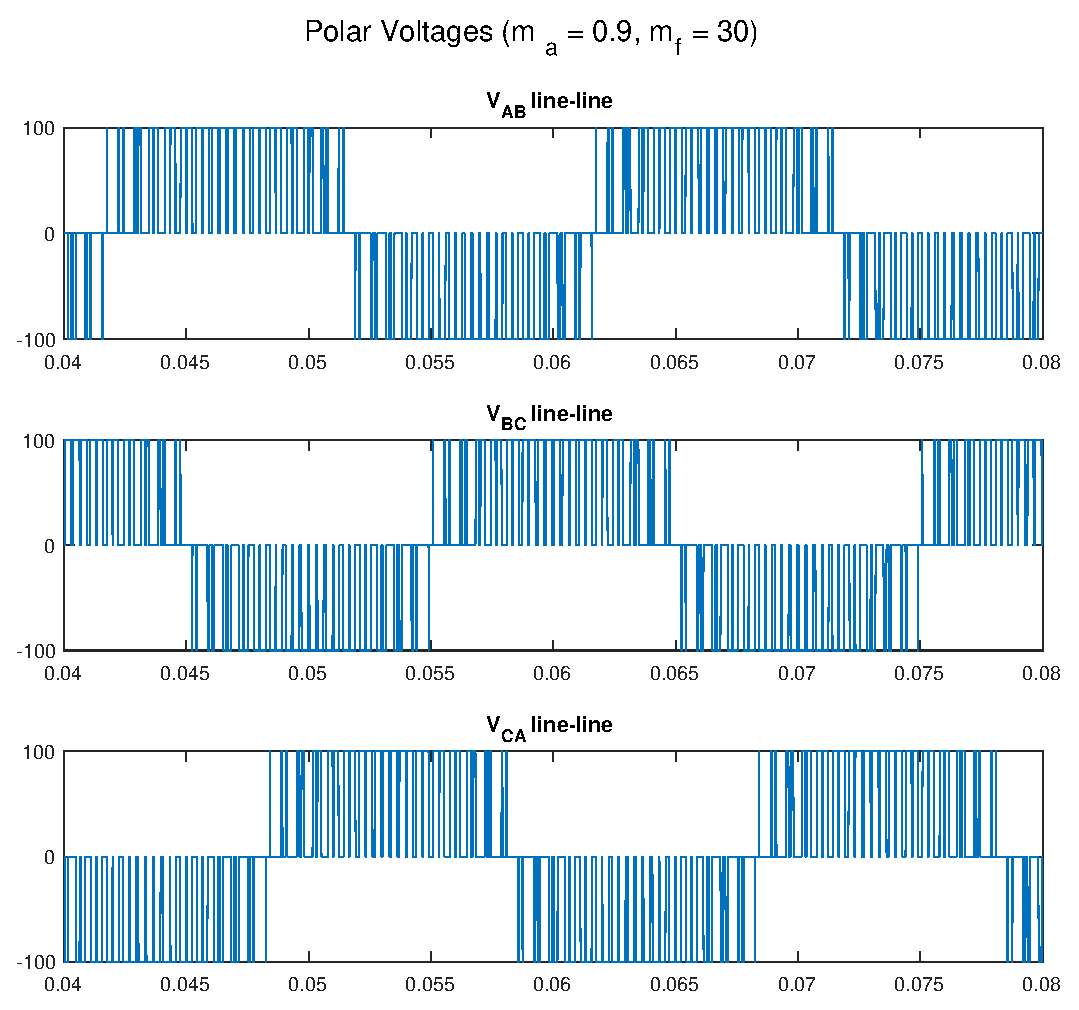
\includegraphics[width=0.95\textwidth]{Images/4_Polar_voltages_30.eps}
	\end{subfigure}
	\begin{subfigure}{0.49\textwidth}
		\centering
		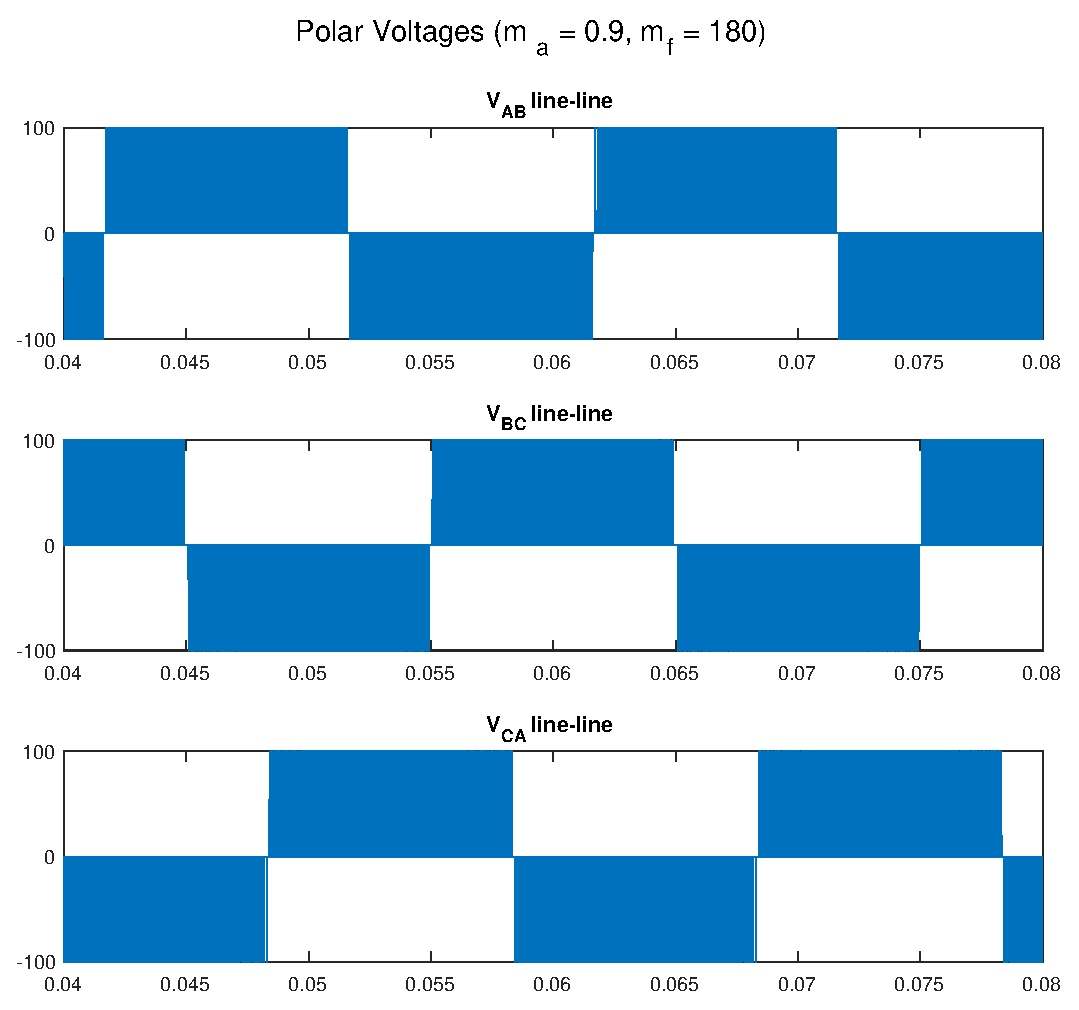
\includegraphics[width=0.95\textwidth]{Images/4_Polar_voltages_180.eps}
	\end{subfigure}
\end{figure}
\noindent
Όπως φαίνεται στα διαγράμματα από πάνω οι πολικές τάσεις εξόδου έχουν πλάτος $V_{dc}$ όπως και η μονοφασική PWM 


\subsubsection*{Τάση εξόδου αντιστροφέα}
\begin{figure}[h!]
	\begin{subfigure}{0.49\textwidth}
		\centering
		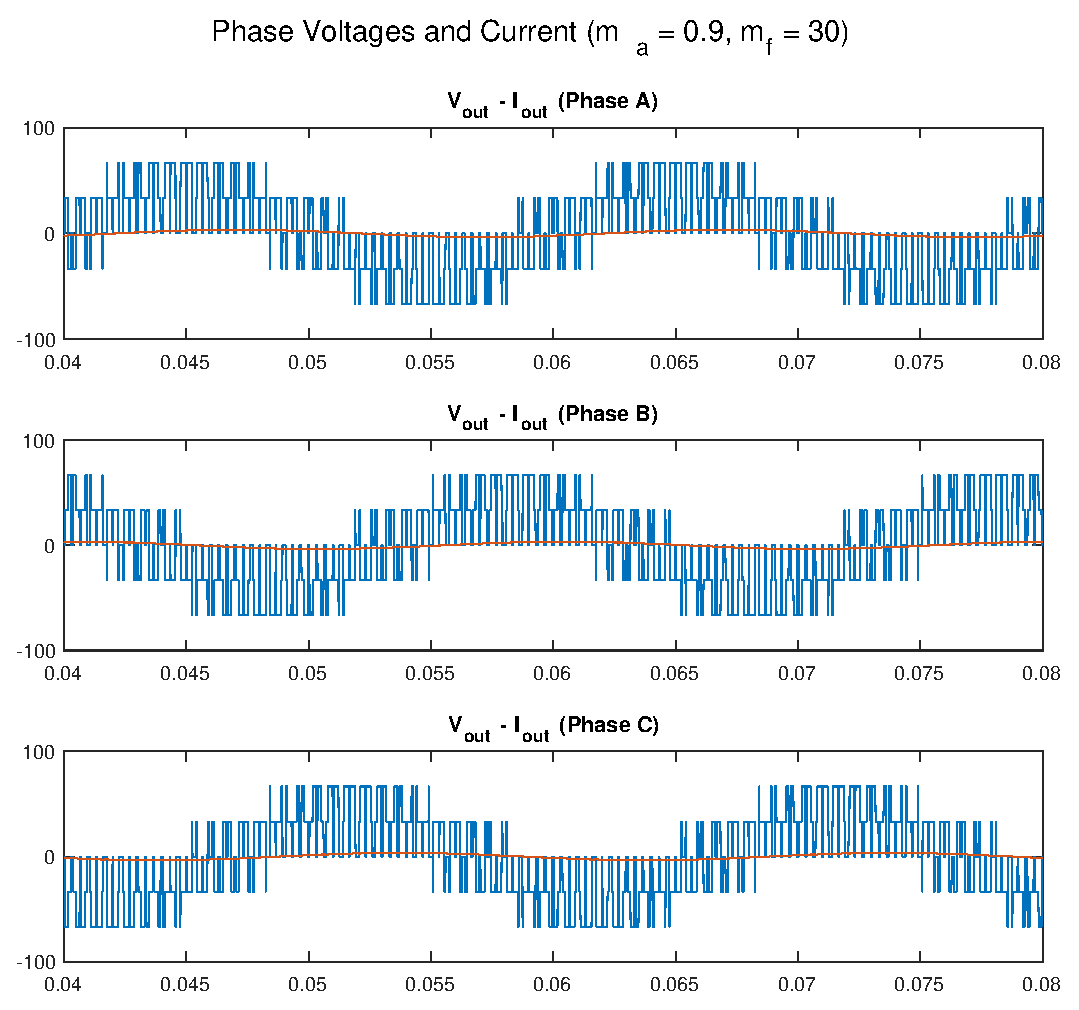
\includegraphics[width=0.95\textwidth]{Images/4_Phase_V_I_30.eps}
	\end{subfigure}
	\begin{subfigure}{0.49\textwidth}
		\centering
		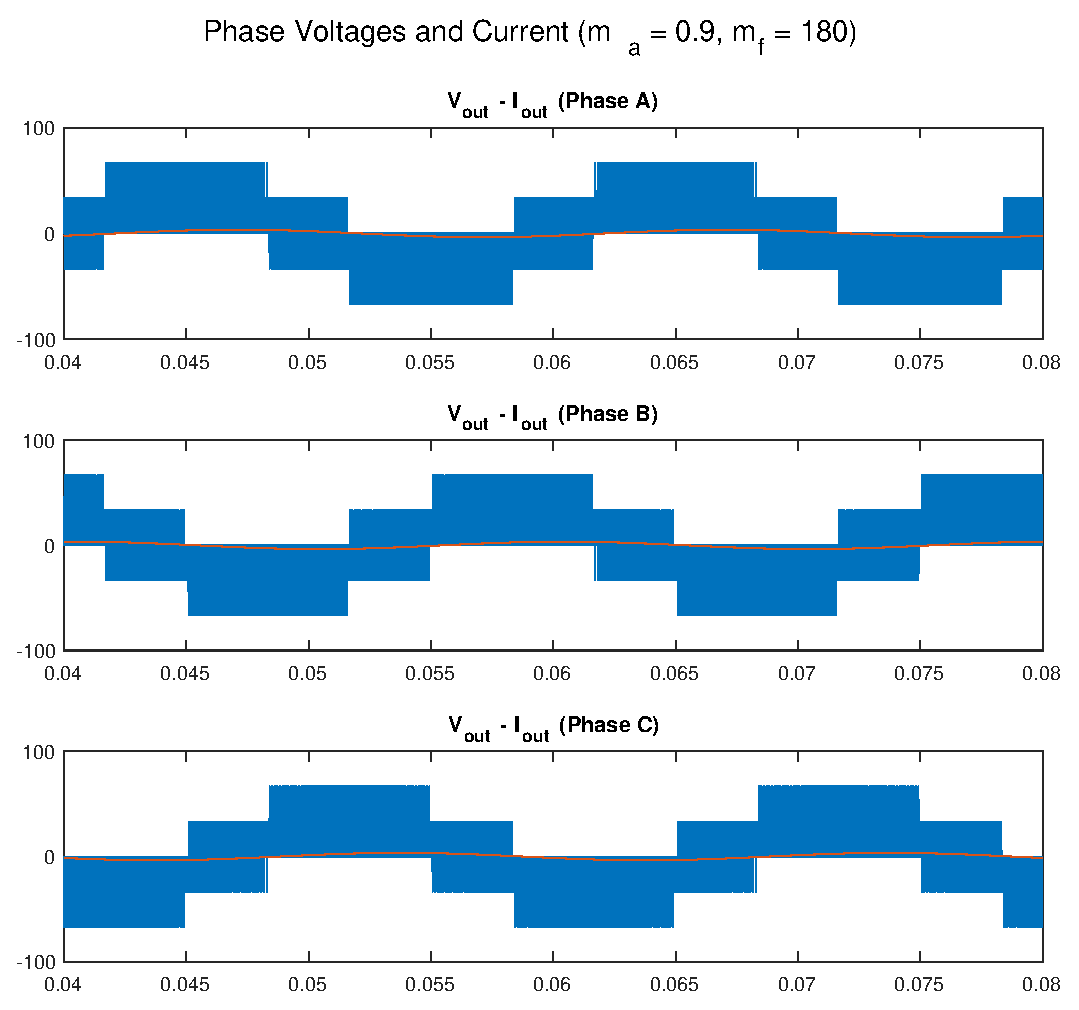
\includegraphics[width=0.95\textwidth]{Images/4_Phase_V_I_180.eps}
	\end{subfigure}
\end{figure}
\noindent
Παρατηρείται σύμφωνα με τα γραφήματα ότι η τάση εξόδου έχει το ίδιο πλάτος και σχήμα και στις δύο περιπτώσεις $m_f$. Όμως στην τάση εξόδου που αντιστοιχεί σε $m_f=180$ παρατηρείται μεγάλη αύξηση της συχνότητας. Ο λόγος αυτής της αύξησης είναι γιατί η συχνότητα είναι γραμμικά ανάλογη του $m_f$ έτσι όταν το $m_f$ εξαπλασιάστηκε από 30 σε 180 το ίδιο έπαθε και η συχνότητα τάσης εξόδου.

\clearpage
\subsubsection*{Ρεύμα Εξόδου ααααααααααααααααααααααααααα}
\begin{figure}[h!]
	\begin{subfigure}{0.49\textwidth}
		\centering
		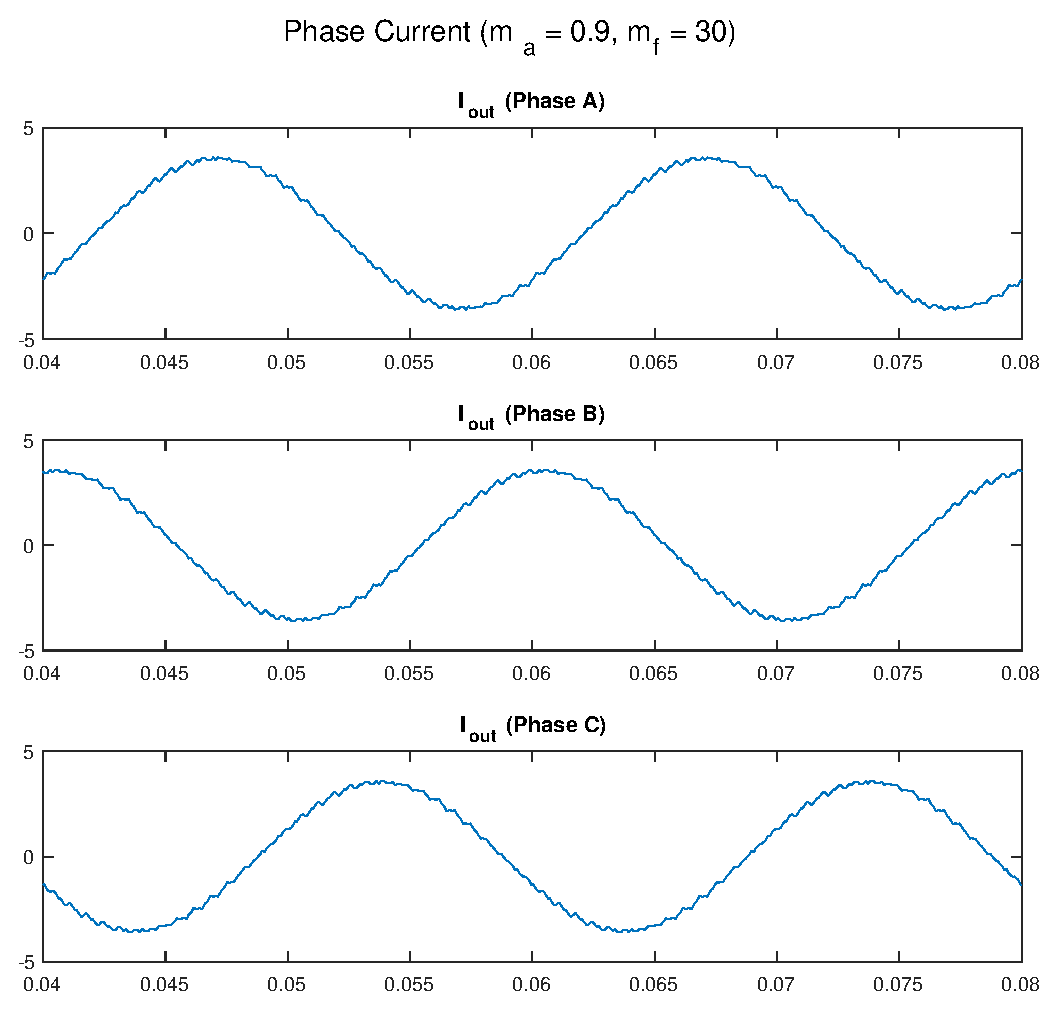
\includegraphics[width=0.95\textwidth]{Images/4_Phase_I_30.eps}
	\end{subfigure}
	\begin{subfigure}{0.49\textwidth}
		\centering
		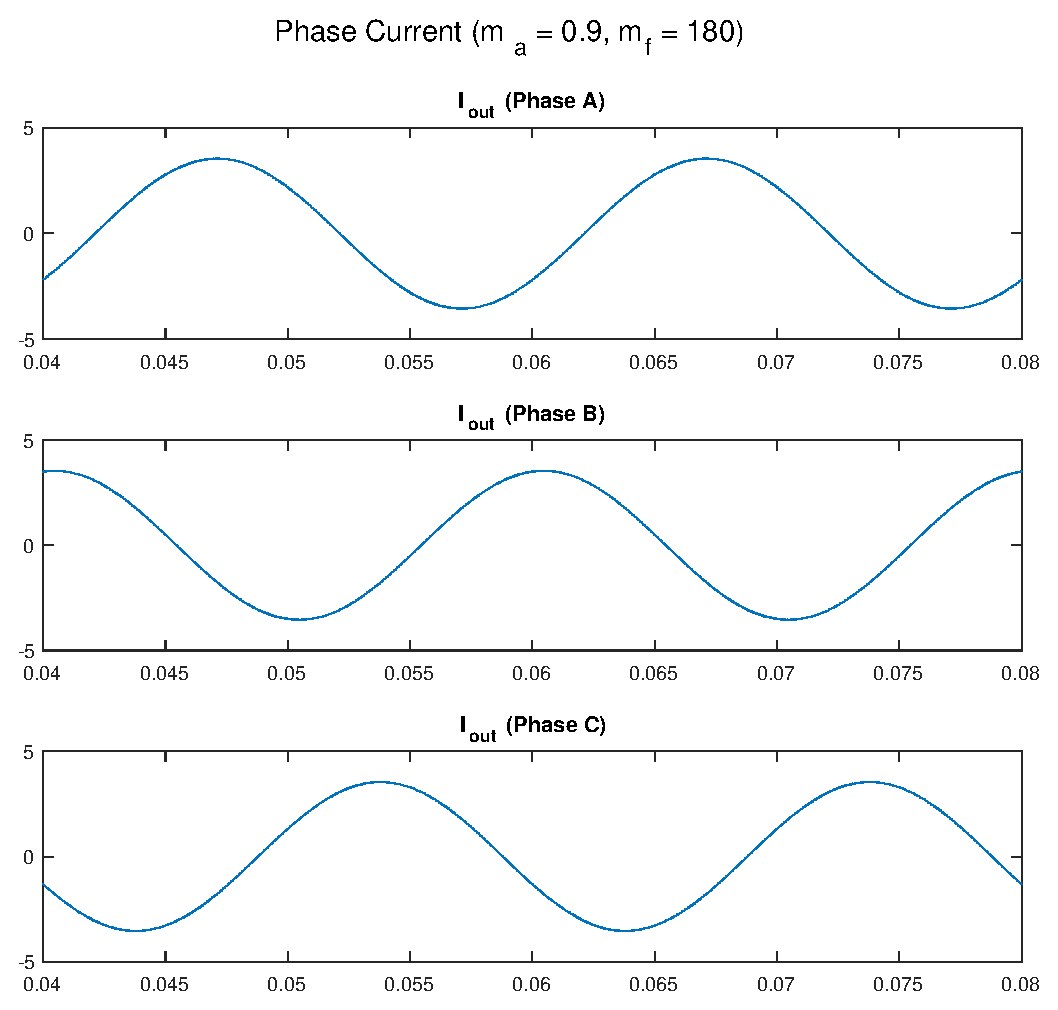
\includegraphics[width=0.95\textwidth]{Images/4_Phase_I_180.eps}
	\end{subfigure}
\end{figure}

\subsubsection*{Ρεύμα διακοπτικών στοιχείων ααααααααααααααααααααααααααα}
\begin{figure}[h!]
	\begin{subfigure}{0.49\textwidth}
		\centering
		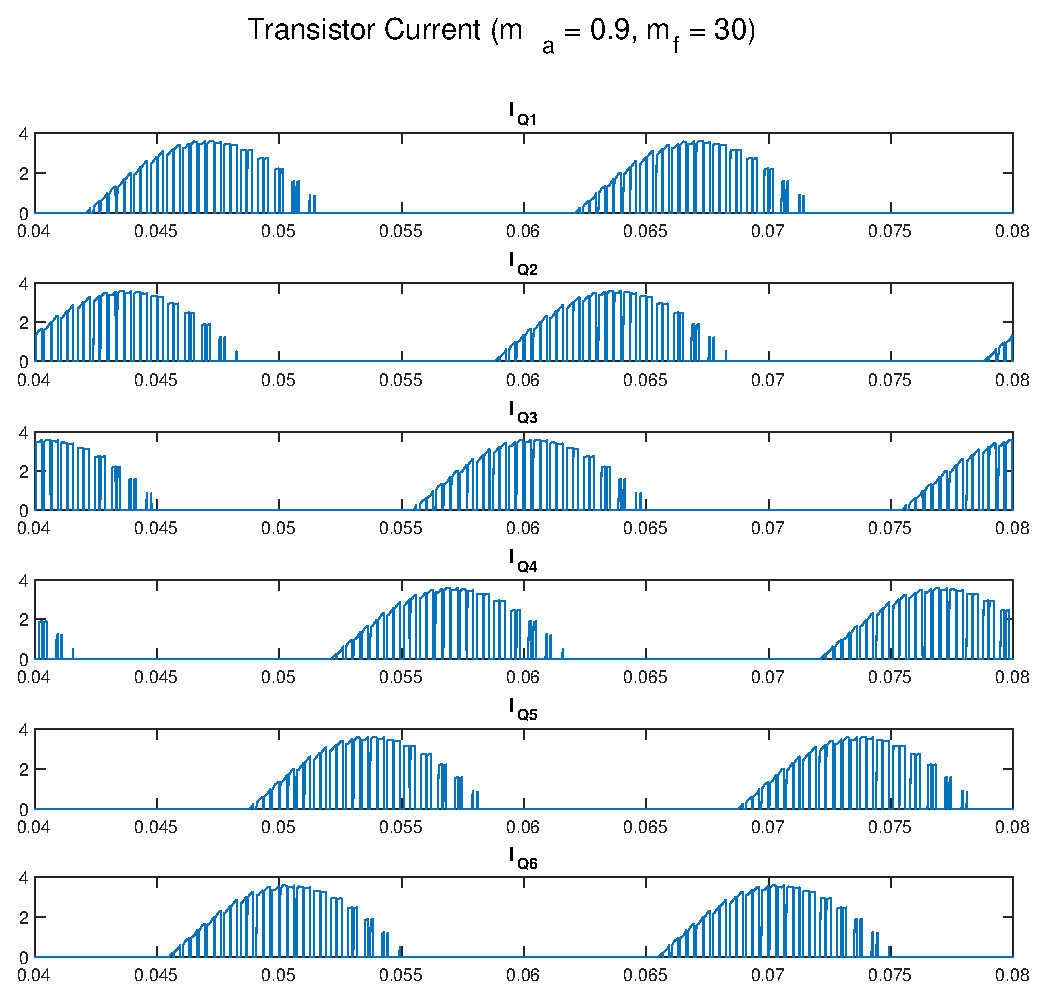
\includegraphics[width=0.95\textwidth]{Images/4_I_Q_30.eps}
	\end{subfigure}
	\begin{subfigure}{0.49\textwidth}
		\centering
		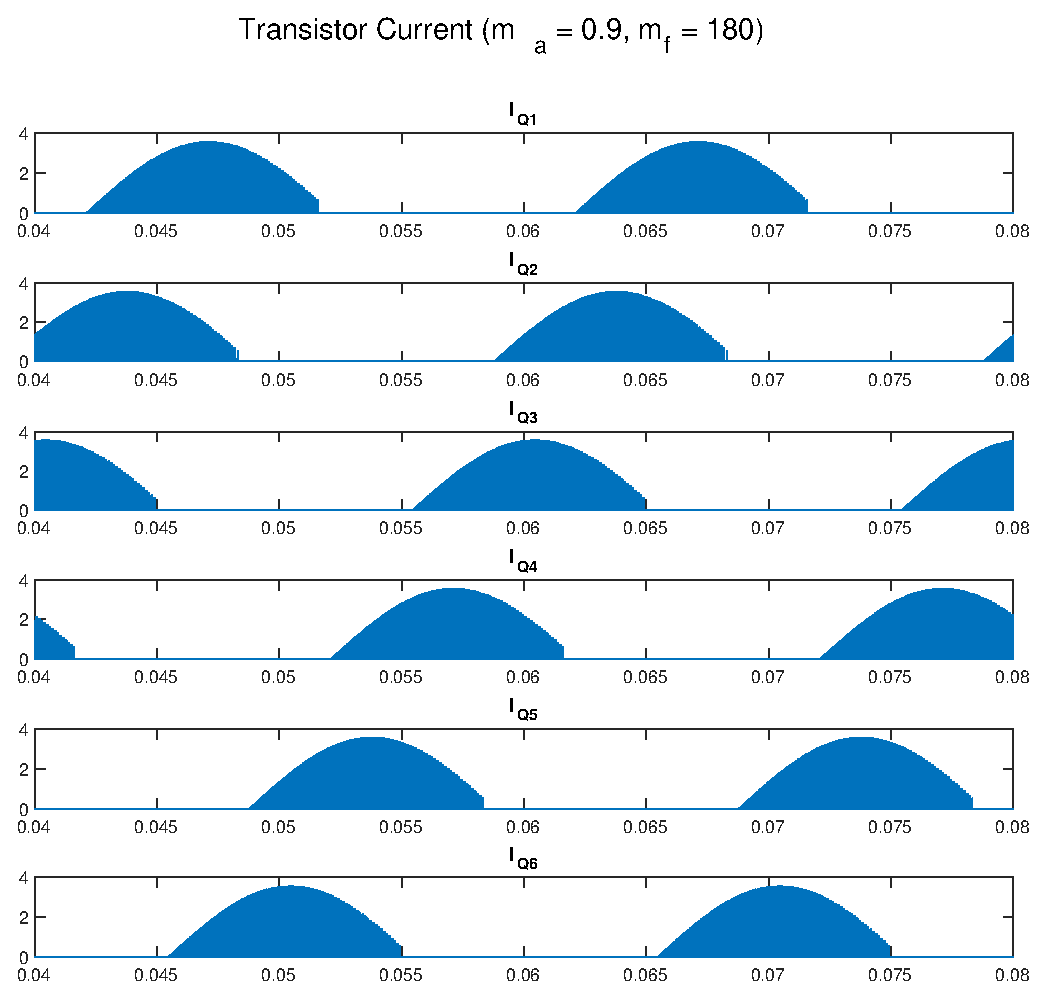
\includegraphics[width=0.95\textwidth]{Images/4_I_Q_180.eps}
	\end{subfigure}
\end{figure}

\begin{figure}[h!]
	\begin{subfigure}{0.49\textwidth}
		\centering
		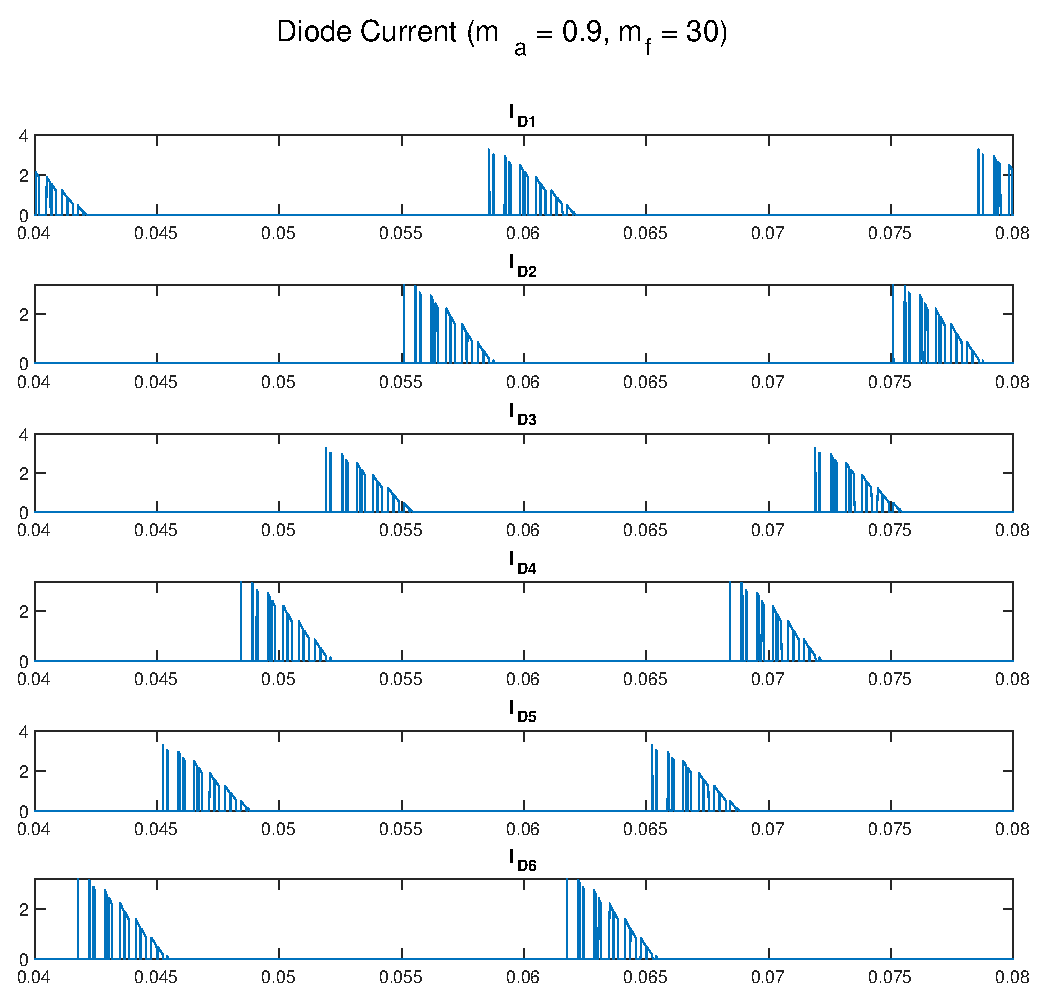
\includegraphics[width=0.95\textwidth]{Images/4_I_D_30.eps}
	\end{subfigure}
	\begin{subfigure}{0.49\textwidth}
		\centering
		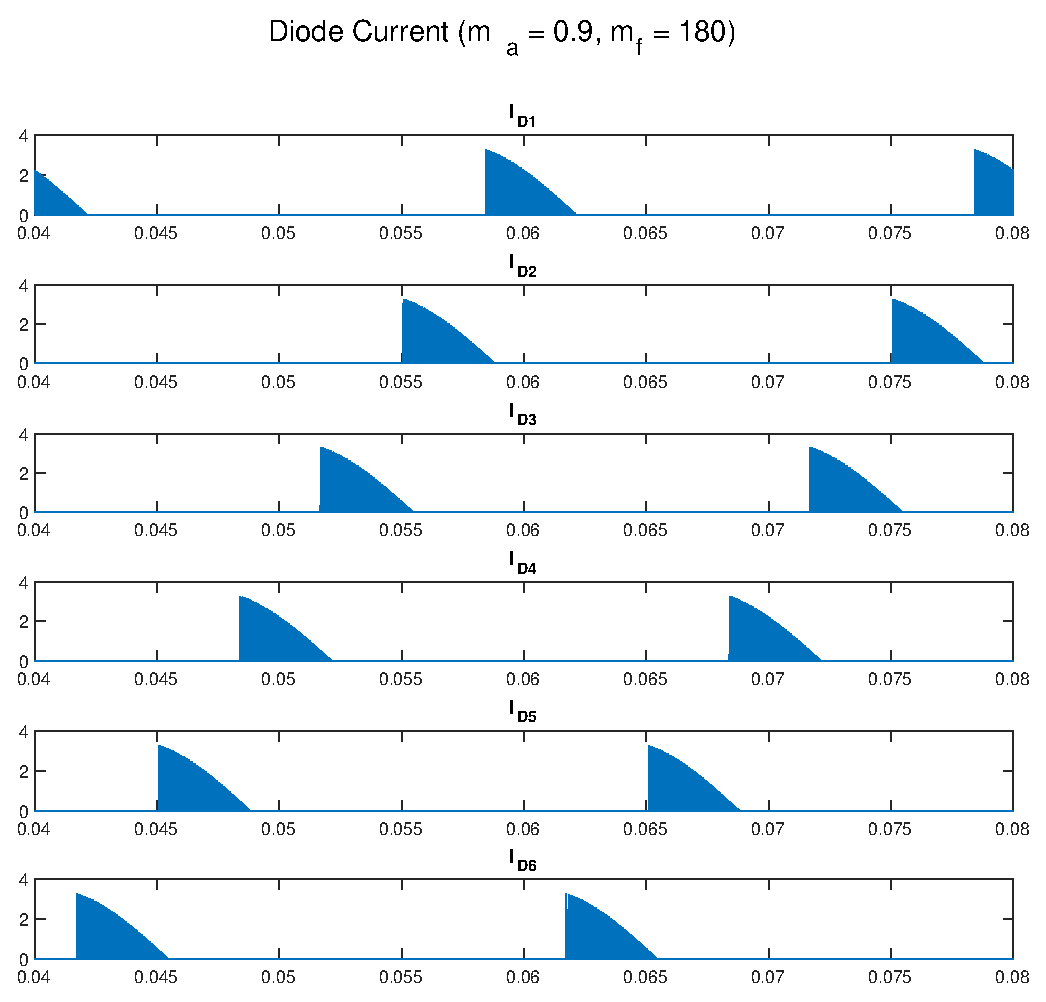
\includegraphics[width=0.95\textwidth]{Images/4_I_D_180.eps}
	\end{subfigure}
\end{figure}
\noindent
Τα διακοπτικά στοιχεία άγουν όπως έχει προαναφερθεί και ανεξαρτήτως τιμής $m_f$ και το άγων ρεύμα έχει ίδιο πλάτος και σχήμα. Μοναδική διαφορά που παρατηρείται ανάλογα της τιμής $m_f$ είναι η συχνότητα. Η συχνότητα είναι ανάλογη με την $m_f$ και συνεπώς για όσο μεγαλύτερες τιμές της $m_f$ τόσο μεγαλύτερη η συχνότητα ρεύματος των διακοπτικών στοιχείων.

\clearpage
\subsubsection*{Ρεύματα Εισόδου}
Τα ρεύματα εισόδου υπολογιστήκαν μέσω του νόμου ρευμάτων Kirchoff και προκύπτουν σύμφωνα με τον τύπο που φαίνεται παρακάτω

\begin{equation*}
	I_{in} = I_{Q5} + I_{Q3} + I_{Q1} - I_{D5} - I_{D3} - I_{D1}
\end{equation*}
\begin{figure}[h]
	\begin{subfigure}{0.49\textwidth}
		\centering
		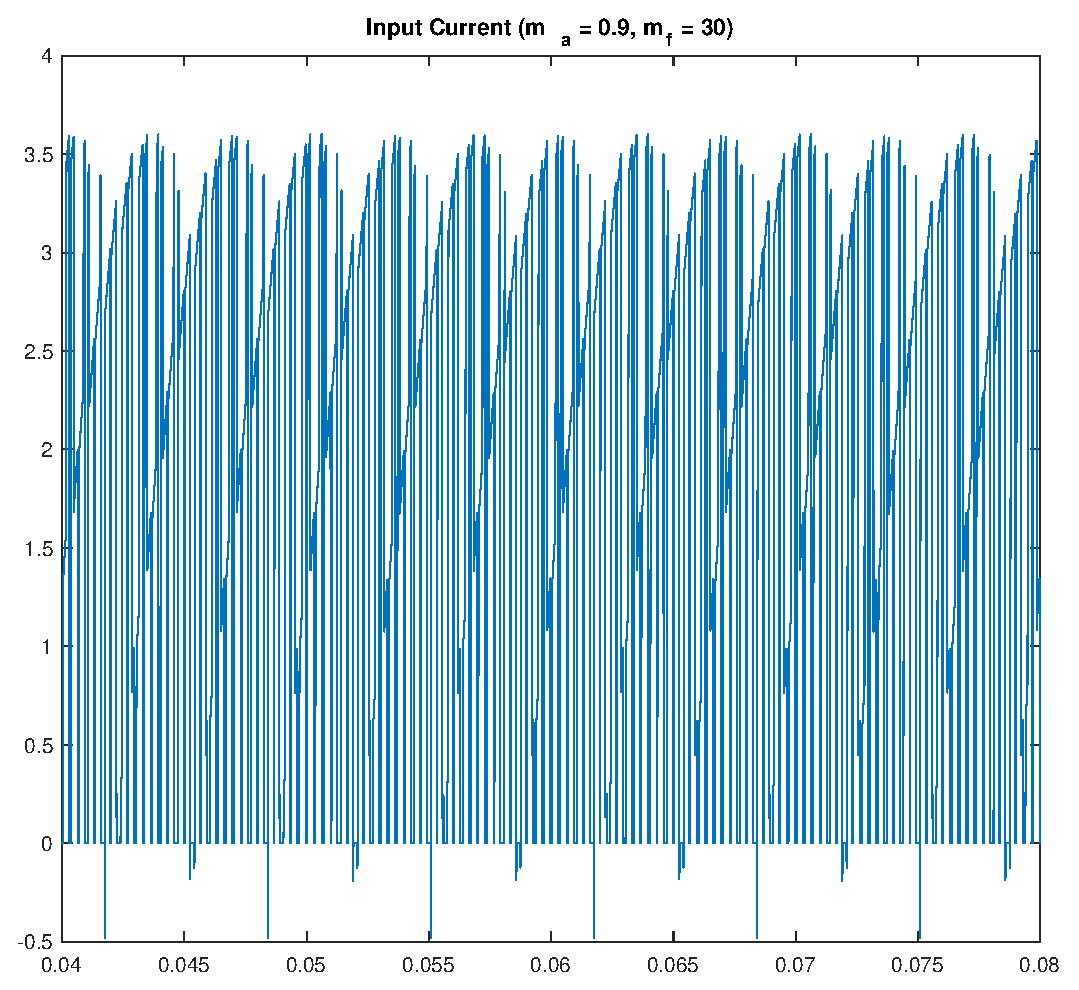
\includegraphics[width=0.95\textwidth]{Images/4_I_in_30.eps}
	\end{subfigure}
	\begin{subfigure}{0.49\textwidth}
		\centering
		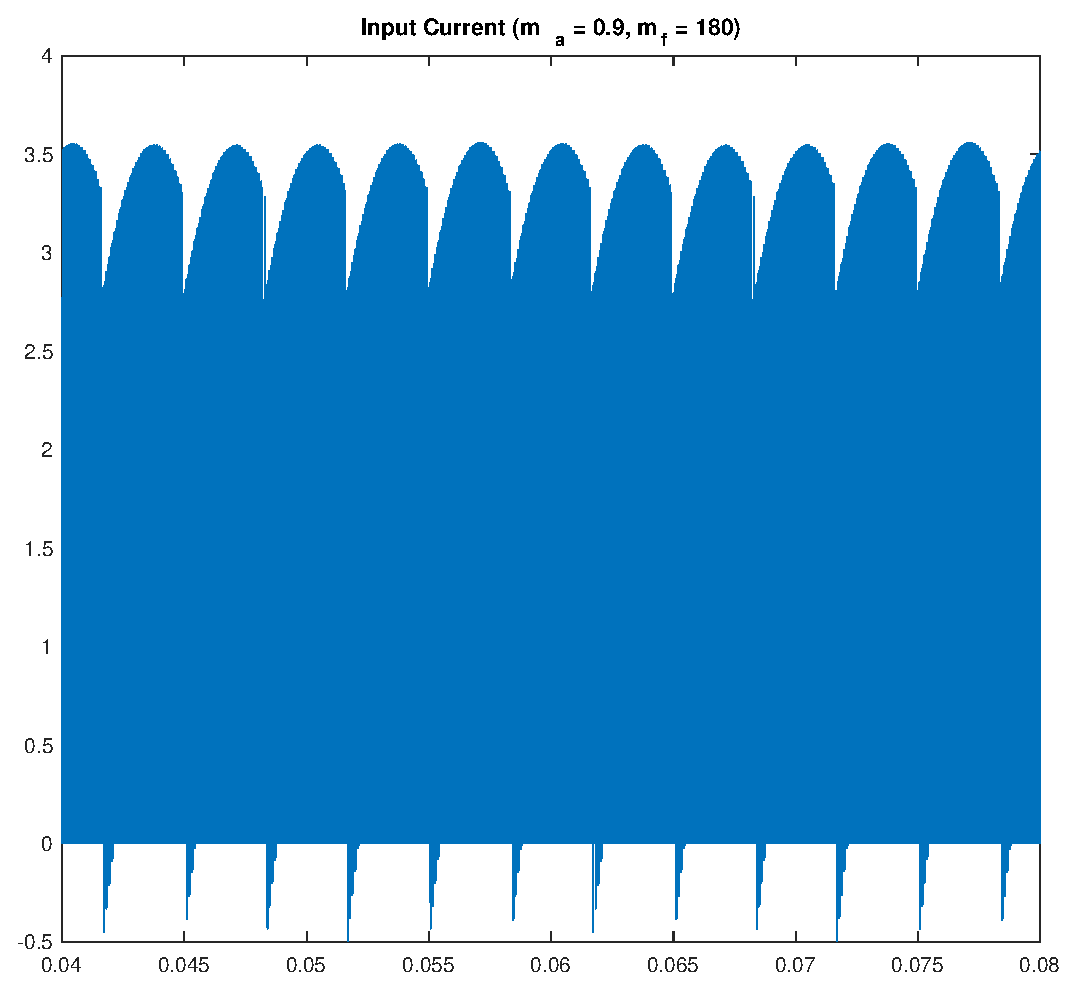
\includegraphics[width=0.95\textwidth]{Images/4_I_in_180.eps}
	\end{subfigure}
\end{figure}

\noindent
Όπως φαίνεται στα παραπάνω σχήματα το πλάτος είναι ελάχιστα μεγαλύτερο στην περίπτωση όπου $m_f=30$ όμως η κύρια ειδοποιός διαφορά των ρευμάτων στις δυο περιπτώσεις είναι η συχνότητα η οποία στην περίπτωση όπου $m_f=180$ είναι κατά πολύ μεγαλύτερη αυτής της περίπτωσης $m_f=30$. Ο λόγος όπως και πριν είναι ότι η συχνότητα είναι ανάλογη με το $m_f$. Τέλος το πλάτος και στις δύο περιπτώσεις είναι κατά ελάχιστα μεγαλύτερο στην πρώτη περίοδο ενώ σταθεροποιείται στις περιόδους που έπονται.

\subsubsection*{Ισχύς}
Η ισχύς εξόδου υπολογίζεται από τον παρακάτω τύπο ενώ η ισχύς εισόδου είναι το γινόμενο τάσης και ρεύματος εισόδου
\begin{equation*}
	P_{out}=V_C\cdot I_C+V_B\cdot \:I_B+V_A\cdot \:I_A
\end{equation*}
\begin{figure}[h]
	\begin{subfigure}{0.49\textwidth}
		\centering
		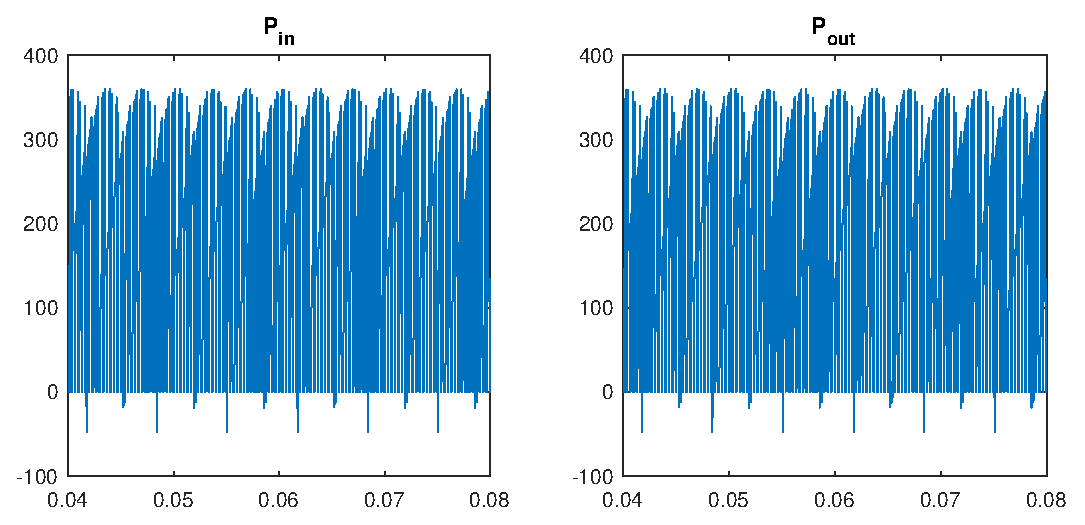
\includegraphics[width=0.95\textwidth]{Images/4_P_30.eps}
	\end{subfigure}
	\begin{subfigure}{0.49\textwidth}
		\centering
		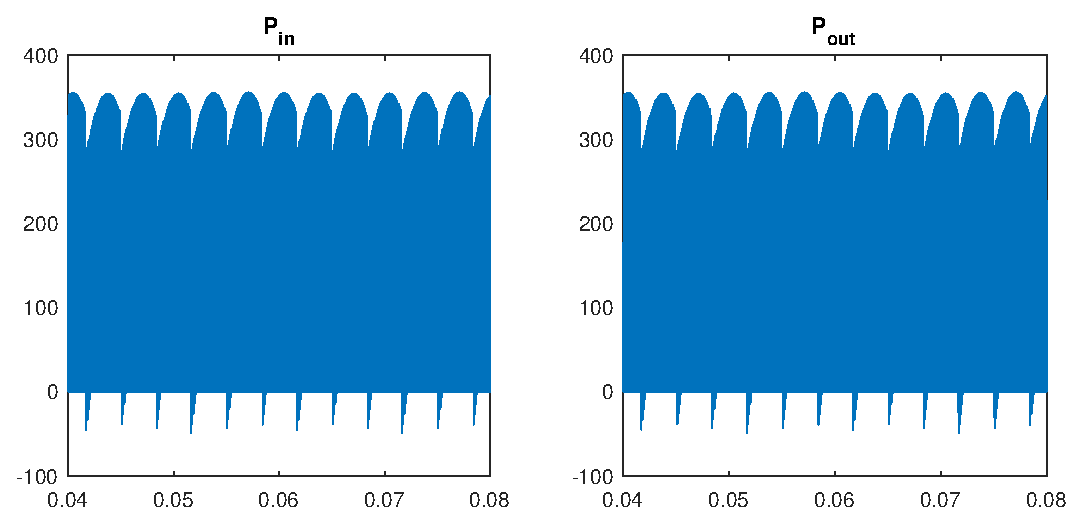
\includegraphics[width=0.95\textwidth]{Images/4_P_180.eps}
	\end{subfigure}
\end{figure}

\noindent
Η ισχύς εισόδου και εξόδου και για τις δύο περιπτώσεις $m_f$ είναι ίδια λόγω της αρχής διατήρησης ενέργειας. Σημειώνεται ακόμη ότι η μορφή της γραφικής της ισχύς είναι ίδια με την μορφή της γραφικής του ρεύματος για την έκαστη περίπτωση και αφού η ισχύς είναι το γινόμενο ρεύματος και τάσης το πλάτος της ισχύς είναι μεγαλύτερο από αυτό του ρεύματος. Ακόμη προφανώς η συχνότητα των ισχύων με $m_f=180$ είναι μεγαλύτερη από την συχνότητα των ισχύων με $m_f=30$ καθώς όπως έχει προαναφερθεί η συχνότητα είναι ανάλογη της $m_f$.

\subsubsection*{Αρμονικές}
Οι αρμονικές εκτός της βασικής αρμονικής βρίσκονται στα σημεία $2\cdot k \cdot m_f \cdot f_1$, όπου κ θετικός ακέραιος αριθμός και $f_1$ η τιμή της πρώτης αρμονικής $f_1=50$Hz
\\\\\noindent
Συνεπώς για $m_f=30$ οι αρμονικές εκτός της βασικής θα βρίσκονται στα σημεία  $2\cdot k \cdot m_f \cdot f_1 = 2\cdot k \cdot 30 \cdot 50 = 3000k$ Αυτά είναι τα σημεία 3000Hz, 6000Hz, 9000Hz κτλ
\\\\\noindent
Ομοίως για $m_f=180$ οι αρμονικές εκτός της βασικής θα βρίσκονται στα σημεία  $2\cdot k \cdot m_f \cdot f_1 = 2\cdot k \cdot 180 \cdot 50 = 9000k$ Αυτά είναι τα σημεία 9000Hz, 18000Hz, 27000Hz κτλ


\subsubsection*{Συντελεστής ισχύος}
Η τιμή του συντελεστή Ισχύος προκύπτει από τον παρακάτω τύπο:
\begin{equation*}
	PF=\frac{P}{S}=\frac{R\cdot \left(I^2_{a,\:rms}+I^2_{b,\:rms}+I^2_{c,\:rms}\right)}{V_{C\:,\:rms}\cdot \:I_{c\:,\:rms}+V_{B\:,\:rms}\cdot \:\:I_{b,\:rms}+V_{A,\:rms}\cdot \:\:I_{a,\:rms}}
\end{equation*}

\noindent
Για να γίνει υπολογισμός σε μια σταθερή κατάσταση επιλέχθηκε αυθαίρετα η 5η περίοδος(?????? ALAZEI ANALOGA ME TON KODIKA) και σε με αυτή υπολογίστηκε ο συντελεστής ισχύος για τις δύο περιπτώσεις των α ως εξής:

\[ 
PF= \left\{
\begin{array}{ll}
	0.6155 & ,m_a=0.9 m_f=30 \\
	0.6154 & ,m_a=0.9 m_f=180 \\
\end{array} 
\right. 
\]

\noindent
Παρατηρείται ότι ο συντελεστή ισχύος για $m_f=30$ είναι ελάχιστα μεγαλύτερος από τον συντελεστή για $m_f=180$. Αυτό οφείλεται στο γεγονός ότι το ρεύμα και η τάση έχουν μεγαλύτερο πλάτος για μικρότερες τιμές του α όπως φαίνεται και στα διαγράμματα ισχύος.
